% #####################################################
% MiToBo User/Developer Manual
%
% File:               MiToBoManual.tex
% Author:             Birgit Moeller
% Date:               13.11.2009
% last update:        20.10.2010
% #####################################################

%  #[ style settings :

\documentclass[11pt,a4paper,english]{report}

\usepackage{amsmath}                   %% mathmatical symbols and formulas
\usepackage[english]{babel}             %% german special signs
\usepackage{epsfig}
\usepackage{fancyheadings}             %% headings and footer
%\usepackage{german}                    %% german speech characteristics
\usepackage{graphics}                  %% inclusion of graphics
\usepackage{graphicx}                  %%     "       "      "
%\usepackage{inputenc}          %% latin-1-coding
\usepackage{listings}
\usepackage{color}
\usepackage{subfigure}
\usepackage{framed}
%\usepackage{../styles/hangcaption}
\usepackage{url}
%\usepackage{hyperref}
\usepackage[pdfpagelabels,linktocpage,breaklinks]{hyperref}
%\usepackage[T1]{fontenc}
\usepackage{xspace}
\usepackage{wrapfig}
%\usepackage{framed} 

% margins
\evensidemargin = -1.5cm
\oddsidemargin = 0.0cm
\textheight 23cm 
\textwidth 16cm
\topmargin -0.75cm
\headsep 1cm
\footskip 1.5cm

%\parindent0pt                          %% no indent of new paragraphs
\renewcommand{\baselinestretch}{1.2}   %% big lineskips

\frenchspacing                         
\sloppy                                %% newlines

\setcounter{tocdepth}{3}               %% depth of table of contents

\setlength\parskip{\medskipamount}     %% line skippings
\parskip1.5ex plus 0.5ex minus 0.5ex   %%

% standard headings and footer
\pagestyle{fancy}
\lhead[\fancyplain{}{}]{\fancyplain{}{}}
\rhead[\fancyplain{}{}]{\fancyplain{}{}}
\lfoot[\fancyplain{\thepage}{\thepage}]{\fancyplain{}{}}
\cfoot[\fancyplain{}{}]{\fancyplain{\thepage}{\thepage}}
\rfoot[\fancyplain{}{}]{\fancyplain{}{}}

% \makeatletter
% \def\@evenhead{
%  \vbox{\hbox to\hsize{\footnotesize \sl \leftmark \hfill }
%  \vspace{10pt} \hbox to\hsize{\hrulefill}}}
% \def\@oddhead{
%  \vbox{\hbox to\hsize{\footnotesize \hfill \sl \rightmark}
%  \vspace{10pt} \hbox to\hsize{\hrulefill}}}
% \def\@evenfoot{\vbox{ \hbox to\hsize{}
%  \vspace{0pt} \hbox to\hsize{\thepage \hfill \sl}}}
% \def\@oddfoot{\vbox{ \hbox to\hsize{}
%  \vspace{0pt} \hbox to\hsize{\sl \hfill \rm \thepage}}}
% \makeatother

% small captions
\makeatletter
\renewcommand{\fnum@figure}[1]{\small\figurename~\thefigure:}
\makeatother

\makeatletter
\renewcommand{\fnum@table}[1]{\small\tablename~\thetable:}
\makeatother

% change footnote color to black
\makeatletter
 \newcommand{\org@footnotemark}{}
 \let\org@footnotemark\@footnotemark
 \def\@footnotemark{%
   \begingroup
    \hypersetup{linkcolor=black}%
     \org@footnotemark
  \endgroup} 
\makeatother

\hypersetup{
  a4paper,
  colorlinks=true,
%  colorlinks=false,
  linkbordercolor=1 1 1,
  urlbordercolor= 1 1 1,
  citecolor=blue,
  %citecolor=black,
  pagecolor=magenta,
  %pagecolor=black,
%  urlcolor=blue
  urlcolor=blue,
  anchorcolor=blue,
  filecolor=black,
  linkcolor=blue
}


\newcommand{\mitobo}{{\bf \tt MiToBo}\xspace}
\newcommand{\mtbimg}{\texttt{MTBImage}}
\newcommand{\imgplus}{\texttt{ImagePlus}}
\newcommand{\imgproc}{\texttt{ImageProcessor}}
\newcommand{\mtbc}{{\bf \tt chipory}\xspace}
\newcommand{\chipory}{{\bf \tt chipory}\xspace}
\newcommand{\alida}{{\bf \tt Alida}\xspace}


\newcommand{\TODO}[1]{\textit{#1}}
\renewcommand{\TODO}[1]{}
\newcommand{\future}[1]{\textcolor{green}{{\footnotesize Future: }#1}}
\newcommand{\tobeimplemented}[1]{\textcolor{blue}{{\footnotesize ToBeImplemented: }#1}}
\newcommand{\designissue}[1]{\textcolor{red}{{\footnotesize DesignIssue: }#1}}

%%%% layout
\newcommand{\itemseparation}[1]{\parskip#1\topsep#1\partopsep#1%
    \parsep#1\itemsep#1}

%%%% lstlisting
\lstset{language=Java, columns=flexible, tabsize=2, numbers=left}



%  #]  :

\begin{document}

%  #[ title page :

\thispagestyle{empty}

\begin{flushleft}
\large{Martin Luther University Halle-Wittenberg} \\
\normalsize{Institute of Computer Science} \\
\normalsize{Pattern Recognition and Bioinformatics}
\end{flushleft}

\vspace*{1cm}

\hrulefill

\vspace*{2cm}

\begin{center}

\large{User and Programmer Guide} \\
\vspace*{0.5cm}

  \begin{figure}[htbp]
    \centering
     
\includegraphics[width = 5cm]{../images/MiToBo_logo.pdf}
  \end{figure}
%\vspace*{-0.5cm}
\Large{
MiToBo - Microscope Image Analysis Toolbox 
}

\vspace*{0.7cm}

\large{
Version 1.0
}
\vspace*{0.5cm}

\normalsize{written by}\\
\vspace*{1.0cm}
\large{The MiToBo Development Team}\\
\vspace*{1.0cm}
\end{center}

\begin{center}
{\Large
{Markus Gla\ss} \hspace*{1cm} {Oliver Gre\ss} \hspace*{1cm} {Danny Misiak}\\[1cm]
       {Birgit M\"oller} \hspace*{1cm} {Stefan Posch} 
}
\end{center}

\newpage
\thispagestyle{empty}
\parindent0pt
%==================================
%Licensing information and copyright
%==================================
{\large \textbf{Licensing information.}}\\[0.5cm]
This manual is part of \mitobo\ - the Microscope Image Analysis
Toolbox.\\[0.5cm]
Copyright \copyright\ 2010-2015\\[0.5cm]
This program is free software: you can redistribute it and/or modify
it under the terms of the \href{http://www.gnu.org/licenses/gpl-3.0.html}{GNU
General Public License
version
3}\footnote{\href{http://www.gnu.org/licenses/gpl-3.0.html}{http://www.gnu.org/licenses/gpl-3.0.html}}
as published by the \href{http://www.fsf.org/}{Free Software
Foundation}\footnote{\href{http://www.fsf.org/}{http://www.fsf.org/}}, either
version 3 of the License, or (at your option) any later version.\\ 
You should have received a copy of the GNU General Public License along with this guide.\\
If not,
see \href{http://www.gnu.org/licenses/}{http://www.gnu.org/licenses/}.\\[1.0cm]
Fore more information on \mitobo\ visit
\href{http://www.informatik.uni-halle.de/mitobo/}{
http://www.informatik.uni-halle.de/mitobo/}.\\[5.0cm] 

{\large \textbf{\mitobo\ is a project at the Martin Luther University
Halle-Wittenberg, \\ Halle (Saale), Germany.}}\\[0.5cm]

\textbf{Institution:}\\[0.5cm]
Institute of Computer Science\\
Faculty of Natural Sciences III\\
Martin Luther University Halle-Wittenberg\\
Von-Seckendorff-Platz 1, 06120 Halle, Germany\\\\
\textbf{Contact:} mitobo@informatik.uni-halle.de\\
\textbf{Webpage:} www.informatik.uni-halle.de/mitobo
\parindent20pt
\newpage
\pagenumbering{roman}


\tableofcontents

%\listoffigures

%\listoftables

%  #]  :

%  #[ main part :

\chapter{Welcome to MiToBo!}
\pagenumbering{arabic}
\label{chap:welcome}
\vspace*{-1cm}
\href{http://rsbweb.nih.gov/ij/}{ImageJ}\footnote{%
ImageJ -- {\em Image Processing and Analysis in Java},
\href{http://rsbweb.nih.gov/ij/}{http://rsbweb.nih.gov/ij/}}
is a widely-used Java toolkit for image processing and analysis. Particularly
in biomedical applications ImageJ has gained large
interest. ImageJ provides the user with a flexible graphical user
interface (GUI), with a large variety of basic built-in image processing operations,
and also with a huge collection of optional plugins downloadable from the
web. From a programmer's point of view, however, the ImageJ API provides less flexibility
to support plugin and application development. Especially easy data access
and exchange between more complex plugins below the GUI appear worth to be improved.

The ImageJ development project {\em ImageJDev }\footnote{ImageJDev website, 
\href{http://developer.imagej.net/}{http://developer.imagej.net/}}
is working towards a new release of ImageJ, {\em ImageJ $2.0$}, 
which is supposed to overcome many of these shortcomings of ImageJ on the programming level. 
The project developers are working on a complete restructuring of ImageJ's system architecture to 
decouple algorithms and user interfaces, and to allow for a much larger flexibility with regard to 
customizing ImageJ's core to specific needs\footnote{To differentiate between both versions of ImageJ throughout the remainder
of this guide, we will refer to the old release simply as 'ImageJ', and to the new version of the ImageJDev project as ImageJ $2.0$.}. 

\mitobo, which is the {\em {\bf \em M}icroscope {\bf \em I}mage Analysis {\bf \em To}ol{\bf \em Bo}x} 
developed at the Martin Luther University Halle-Wittenberg, targets at manifold goals. 
On the one hand it seeks to enhance the functionality and usability of ImageJ for programmers and users.
It shares the goals of an improved API and a strict decoupling of algorithmic 
functionality and user interfaces with the ImageJDev project. For example, \mitobo and ImageJ $2.0$ 
both define unified frameworks for implementing new functionality in terms of plugins and operators,
respectively, and both systems support the automatic generation of graphical user interfaces from 
these implementations.

On the other hand, however, \mitobo 
offers additional functionality going behind the features of ImageJ $2.0$.
With regard to graphical user interfaces it not just supports the automatic generation of user 
interfaces for single operators or plugins, respectively. 
Rather it extends the underlying model of image analysis procedures towards {\em workflows} 
where multiple operators are sequentially or in parallel applied to given input data for 
extracting desired results. 
This extension is inherently included in \mitobo's core and available to the user in 
terms of a graphical editor named {\bf \em Grappa} (Sec.~\ref{sec:grappa}) which supports users in designing workflows.
  
In general and contrary to the ImageJDev project \mitobo not only focusses on graphical user 
interfaces, but provides mature functionality for assessing implemented algorithms from commandline 
as well. In addition, it features a built-in mechanism for automatic documentation of analysis 
procedures which significantly simplifies the reconstruction of results and their long-term archival.
Finally, \mitobo not only inherently provides a comfortable framework for developing and 
implementing new image analysis algorithms. The toolbox also includes a selected collection of common image 
analysis techniques. They are mainly dedicated to the area of biomedical image analysis, but not restricted
to this field. Among these algorithms are for example segmentation approaches based on active 
contours for cell and scratch assay images, tools for neuron image analysis, or wavelet-based 
algorithms for detecting subcellular structures.

\mitobo is fully compatible with ImageJ, and features prototypical support for ImageJ $2.0$
which, however, will soon be completed towards full support. \mitobo's operators can be used both from 
within ImageJ and ImageJ $2.0$. In addition, \mitobo is capable of executing plugins from ImageJ 
$2.0$ and, e.g., include them in its process documentation. \mitobo is licensed under GPL, version
$3$, and can be downloaded from its website 
\href{http://www.informatik.uni-halle.de/mitobo}{http://www.informatik.uni-halle.de/mitobo}.
Please also have a look at the website for installation instructions.

\section{\mitobo's Core: Alida}
\mitobo's main paradigm is the idea of completely decoupling the implementation of functionality
from corresponding user interfaces for making this functionality available to users. The strict 
separation of algorithms and potential user interfaces offers largest flexibility to programmers.
It releases them from the cumbersome task to explicitly implement a variety of different interfaces.
At the same time the programmers are guided in implementing new functionality by clearly defined 
specifications and interfaces from which also users benefit. The usage of implemented 
functionality gets significantly simpler as the user interfaces for different algorithms follow 
common principles with regard to structure, appearance and handling.    

\mitobo\ is build on top of
\href{http://www.informatik.uni-halle.de/alida}{\alida}\hspace{-0.15cm}\footnotemark[4]
\footnotetext[4]{Alida website, \href{http://www.informatik.uni-halle.de/alida}{http://www.informatik.uni-halle.de/alida}}
from which it inherits the functionality for automatic user interface generation and automatic
documentation of analysis processes. \alida, which is the acronyme for 
{\em {\bf \em A}dvanced {\bf \em L}ibrary for {\bf \em I}ntegrated {\bf \em D}evelopment of 
Data Analysis {\bf \em A}pplications}, is a framework for supporting programmers in developing 
data analysis applications. It ships as a library providing core functionality for implementing
so-called {\em operators} as functional units for data analysis, and which also subsumes handy 
applications for running operators in a graphical or commandline context, as well as the graphical workflow editor {\bf \em Grappa}.

\alida basically interprets each data analysis pipeline as a 
process of modifying given input data (not necessarily image data) by a series of operations to produce the desired output data. 
Accordingly, all data analysis procedures in \alida\ are implemented by {\em operators} which are the only places to manipulate 
data. Furthermore, operators can be combined into {\em workflows}. 
Each workflow consists of a set of operators executed sequentially, in parallel or in a
nested fashion. Particularly the latter option naturally renders each workflow to form a new 
operator by itself, hence, in \alida a workflow is just an operator with extended functionality.  

It is straightforward to associate a selection of sequential and/or parallel operator calls 
with a directed graph data structure, where each operator is linked to a certain node of the graph, 
and input and output data is passed from one operator to another along the graph edges. This graph
together with the individual configuration parameters of all involved operators is a sufficient base
for lateron reconstructing all steps of data manipulation for a given result data object.
\alida\ allows to extract such {\em history graphs} explicitly and by this offers a powerful tool 
for the automatic documentation of data analysis processes. 
Note that these history graphs are not 
identical to the graphs implicitly defined by workflows as introduced above. 
Rather a workflow graph is often
only a subgraph of the history graph associated with the results generated by executing the 
workflow. This is due to the fact that operators usually rely on internal calls to other operators 
and these calls are not linked to an operator node in the workflow graph.   

\mitobo\ fully adopts the concepts of \alida, i.e.~\alida is an integral part of the \mitobo
framework. Consequently, image analysis procedures are realized in terms of operators which can be 
applied to data objects, e.g., images, regions or image primitives like keypoints and lines, 
and yield certain results. Contrary to \alida, which does not depend on any other data analysis
framework, \mitobo\ builds upon ImageJ. It basically relies on ImageJ's image data types, however,
does not interfere with ImageJ's plugin interfaces. Rather it allows to program ImageJ-compatible 
plugins based on the \alida\ operator concept.
Thus, in addition to the ImageJ interfaces which focus on plugin and script development,
\mitobo\ defines unique interfaces for the underlying image processing modules, i.e.~operators, in
terms of input/output data and parameters, and also with regard to the way how operators can be
invoked from other operators or user interfaces. This significantly improves data exchange and
operator handling, and establishes -- besides the already mentioned concept of automatic 
documentation -- a powerful fundament for adding new sophisticated features to ImageJ and ImageJ 
$2.0$. 

In the remainder of this guide we will outline the core functionality of \mitobo\ and its features with more 
detail. In doing so we will refer to the basic concepts of \alida only in a rudimentary fashion. 
If you are interested in more details about \alida, please refer to the \alida website\footnotemark[4] 
where you can find more information on \alida
bundled with examples of how to implement operators and how to execute them.

\section[\mitobo's Main Features: Operators, History Graphs and User Interfaces]
         {\mitobo's Main Features:\\ Operators, History Graphs and User Interfaces}
\label{sec:features}
\enlargethispage{0.2cm}
Besides providing modern image analysis tools and algorithms for microscope image analysis the
overall goal of the \mitobo\ project is to ease the analysis in terms of the development of appropriate algorithms and flexible user interfaces. These interfaces should, of
course, not only be designed for experts,
but also for researchers using image processing software as a tool rather than
developing their own
algorithms. \mitobo\ builds on top of ImageJ which has achieved large success and broad acceptance by researchers from
many different disciplines who need to solve their individual image analysis
problems. 

From the programmer point of view, ImageJ yields a suitable base for developing
image analysis tools in an integrated
framework. The programmer does not need to take care of, e.g., image display and zooming, as ImageJ
has answered such questions already. However, providing a certain degree of usability and easy integration
of new algorithms in terms of plugins is only one side of the medal. On the
other hand the underlying software
structures and interfaces should also provide a sufficient degree of comfort to the
programmer. In particular, image processing algorithms and user interfaces should be clearly separated from each other and data exchange between
different modules should be easy in terms of well-specified interfaces. 

As ImageJ is not optimally designed with regard to some of these aspects,
\mitobo\ does not exclusively focus on the
development of image analysis tools for microscope images, but also optimizes underlying software
in terms of data flow and data structures. In addition, self-documentation of image processing
pipelines is natively supported.

Based on the underlying concepts of \alida, \mitobo\ defines an image analysis pipeline as a sequence of operations sequentially or in
parallel applied to data that is handed over from operator to operator. Such a pipeline may be
viewed as a directed graph structure, where the nodes represent different operators and the data
flow is indicated by edges in between. From this interpretation of image analysis in
general, several design issues are derived that are embedded in the \alida\ core of
\mitobo. The concepts by themselves as well as functionality build on top of them are an integral part of \mitobo 
and provide users as well as programmers with enhanced image analysis tools and an improved
infrastructure for development and research.

\paragraph{Operator Concept.} The interpretation of image analysis pipelines as a
sequence of operations directly leads to the concept of {\em operators} implemented in \mitobo. 
All manipulations that are performed on data are done by operators. Vice versa operators
are the only actors that work on given data, modify the data or generate new
data entities from given input data. Accordingly, all image processing and
analysis algorithms in \mitobo\ are implemented in terms of operators with clearly specified input and output interfaces.

The operator concept is adopted from \alida. Technically \alida\ defines a common superclass for
data analysis modules denoted '{\tt ALDOperator}' from which the \mitobo\ main operator
class '{\tt MTBOperator}' is derived, and which all \mitobo\ operator classes extend. 
Furthermore, the concept incorporates a formal description of the interface of an operator,
i.e.~a formal specification of its inputs, outputs, and parameters, which is realized by the Java annotation
mechanism. In addition, there is only one possibility to invoke operators which is a single public routine to be
called from external which results in a unified invocation procedure for all operators. Among other things, this 
yields the base for automatic process documentation and user interface generation.
Moreover, every new operator implemented based on \mitobo and following these rules directly benefits from this
infrastructure, i.e.~can generically be executed and is automatically considered in extracting processing graphs.

\paragraph{Automatic Process Documentation and History Graphs.} The \alida\ operator concept with its transparent
interface specifications allows a unified handling of operators in various contexts, e.g., with
regard to graphical programming or automatic or semi-automatic code generation
where compatibility checks and operator calls have to be standardized. In
addition, the restriction of operator invocation to a single available method
also serves as a basis for another sophisticated feature of \mitobo\ which is the
fully automatic
documentation of image analysis pipelines. Given the interpretation of image
analysis pipelines as sequences of operators, all that remains to be done for
process documentation is to log the calls of all operators as well as their input and
output data and save their parameter settings. Together with
information about the order of operator
calls, for example represented in a directed graph data structure, these data
form a complete protocol of the pipeline and allow for longterm documentation of
analysis processes. In particular, linked to specific result data
objects, they allow to reproduce all results ever produced during the course of
algorithm development, testing, or
experimental evaluation.

The concept of automatic process documentation is realized in \alida, thus, it is also an integral part of
\mitobo\ and directly embedded into the operator concept. Operators provide internal functionality to
store process data during the course of an analysis procedure which later on can be extracted in terms of a
{\em history graph} file in XML format. Such a graph is associated with each data object being the
result of a certain operator or sequence of operations. Although the majority of objects will be
images, processing histories can also be associated with
segmentation results like regions or contours as well as histograms or any
other numerical data. See Figure~\ref{fig:DAG} for an example processing graph.

\paragraph{User Interfaces and Workflow Design} For (scientific) programmers the development of new image analysis algorithms
is mainly linked to the implementation of functionality to achieve desired results. For users who would like to 
benefit from new algorithms in their daily work the availability of suitable user interfaces is equally important. 
But as interface design and development usually coincides with a significantly increased amount of time for the programmer 
required to provide users with handy interfaces this aspect is often neglected. 

The unified invocation procedures for operators in \alida and their clear specification of input and output parameters pave 
the way for releasing programmers from the cumbersome task of implementing user interfaces. \alida, and consequently \mitobo,
inherently include mechanisms to automatically generate graphical as well as commandline user interfaces from operators in a 
completely generic fashion. Particularly, \alida's built-in support for a large variety of standard Java datatypes as operator 
parameters as well as for more sophisticated types like arrays, collections or enumerations renders it quite easy to implement
new functionality including suitable user interfaces with a minimum of programming overhead. 

And also users benefit from \mitobo's automatically generated user interfaces. Naturally all interfaces 
follow the same design and handling principles, e.g., all of them provide access to \mitobo's online help or allow for running 
the operator in batch mode. Moreover, \alida and \mitobo not only automatically generate user interfaces for single operators, 
but inherently support also the design of complete workflows formed by multiple operators which only in combination yield 
desired results. The graphical workflow editor {\bf \em Grappa} being shipped with \alida and \mitobo targets at supporting 
users in designing new workflows in a graphical manner. It integrates all operators implemented in the \mitobo framework as 
potential nodes of workflow graphs and allows for linking input and output parameters of these nodes to define more 
complex workflows. Thereby it takes full benefit of \alida's functionality, i.e.~Grappa offers automatically generated graphical
components for node configuration, data compatibility checks on dragging edges, and the fully automatic verification of operator 
configurations at runtime.

\section{About this Guide}
\label{sec:about}
This guide is organized in a short introductory section and two main parts. The introductory
section -- which you most probably have already read in the last few minutes -- is dealing with
some general remarks, while the two main parts provide more details. 
The first part is dedicated to users who are interested in using \mitobo\
plugins or commandline tools for their own work, e.g., to benefit from the automatic process documentation
capabilites of \mitobo or to adopt provided image analysis algorithms for solving their own image
processing problems. 
The second part introduces the reader to some more internals of \mitobo,
i.e.~it presents more details about the operator concept and how to use it with own
code, more information about specific \mitobo\ data types and also about programming with \mitobo\
in general. Note that only some few basics of the underlying concept of \alida\ are presented. 
For more details about its functionality and technical implementation refer
to the \alida\ manual to be found on the \alida\ webpage\footnotemark[4].

We hope that the new perspectives that \alida and in particular \mitobo\ open with 
their concepts might be helpful for developers and users of image processing applications, 
and by this extend ImageJ's selection of valuable features.  
If something remains to be clarified or if you have further notes and comments, just write an email
to us at {\tt mitobo@informatik.uni-halle.de}. We are happy to get in touch with you! 


%==================================
\part{MiToBo: The User's View}
\chapter{Working with \mitobo}
\label{chap:work}
\mitobo ships with a large collection of image analysis operators, basically developed for
microscope image processing and analysis, however, applicable to any other image analysis
task as well. After \mitobo was successfully installed (please refer to its
website, \href{http://www.informatik.uni-halle.de/mitobo}{http://www.informatik.uni-halle.de/mitobo}, for details
on the installation procedure) you can directly use the operators and plugins of the toolbox like any other ImageJ plugin 
(Sec.~\ref{sec:opRunImageJ}). In addition, \mitobo provides a commandline tool for running operators, e.g., from shell scripts
(Sec.~\ref{sec:opRunCmdline}). 
Irrespective of how an operator is invoked, after termination processing histories can be accessed and explored for all result 
data objects (Sec.~\ref{sec:history}). 
Finally, if you require to combine various operators into a more complex workflow for solving your specific problem, the graphical 
editor {\tt Grappa} offers support for doing this in a comfortable graphical manner (Sec.~\ref{sec:grappa}).

\section{Running Operators within ImageJ and ImageJ $2.0$}
After installing the \mitobo jar archive with all its dependencies \mitobo adds a new entry 
denoted 'MiToBo' to ImageJ's plugin menu from where you have access to \mitobo's functionality 
(Fig.~\ref{fig:imageJ}). It basically subsumes an option 'MiToBo Runner' to open \mitobo's 
operator runner which grants access to all \mitobo operators (see below), and an item 
'Grappa Editor' to invoke the graphical workflow editor (Sec.~\ref{sec:grappa}). In
addition, there might appear some more items. All of them are related to so-called 'quick start
plugins'. These ImageJ plugins allow direct access to some interesting operators (and some few
real plugins) in \mitobo 
dedicated to specific applications or techniques. Among those are for example
\begin{itemize}
  \item the {\tt 'Scratch Assay Analyzer'} which is a tool for quantifying gap development in 
  	scratch assay images as used in cell migration experiments \cite{Glass12_PR, Glass12_ImageJ},
  \item the {\tt 'Snake Optimizer'} which features an implementation of parametric active contours
  	and in particular allows for interactive evaluation of various energy models
  	\cite{Moeller12_IJ},
  \item {\tt 'Threshold Image'} which is an interactive image thresholder,
  \item and finally the two plugins {\tt 'Open Image MTB'} and {\tt 'Save Image MTB'} which allow
  	for image I/O considering extracted processing histories (cf.~Chap.~\ref{sec:history}).  
\end{itemize} 
\begin{center}
\begin{figure}[t]
\begin{center}
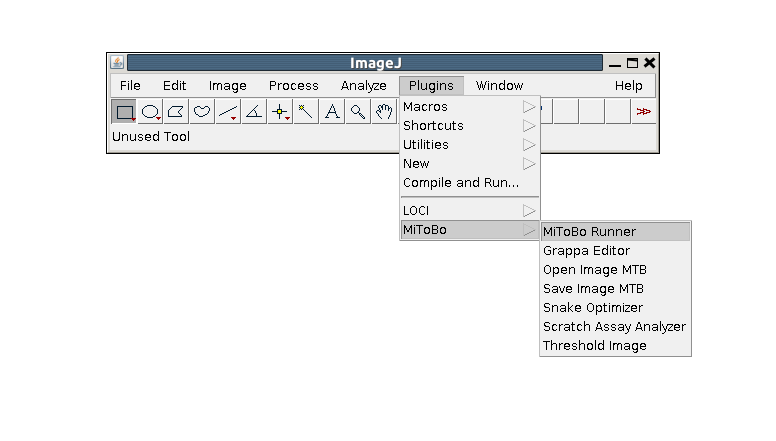
\includegraphics[width=0.85\textwidth,clip,trim= 0 0 0 30]{../images/ScreenshotImageJ_trans.png}
\vspace*{-1.7cm}
\caption{\label{fig:imageJ}Screenshot of ImageJ's plugin menu including \mitobo's submenu.}
\end{center}
\vspace*{-0.25cm}
\end{figure}
\end{center}

\vspace*{-0.75cm}
As mentioned above the key component for accessing \mitobo's functionality from within ImageJ is
its operator runner. Fig.~\ref{fig:oprunner} shows a screenshot of its main window after it has 
been invoked from ImageJ's plugin menu\footnote{\mitobo also offers a toolbar button and an associated start-up macro
to enable direct access to the operator runner, please refer to the installation instructions on the webpage for details on 
how to setup the button.}.

\begin{wrapfigure}[19]{r}{0.5\textwidth}
\vspace*{-1.6cm}
\begin{center}
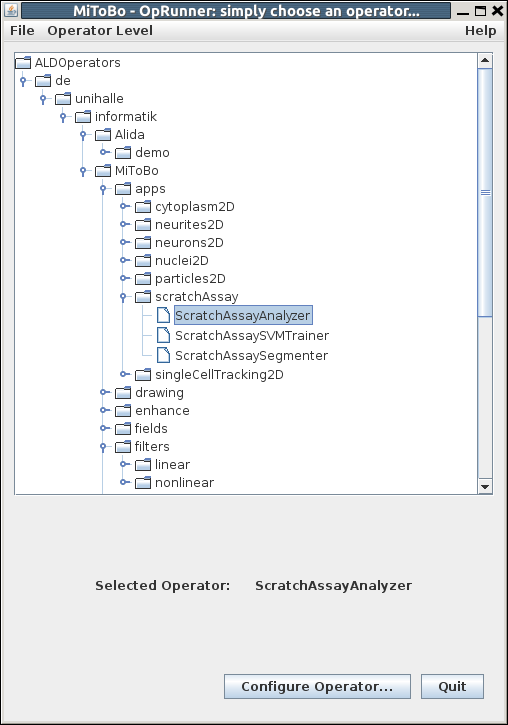
\includegraphics[width=0.475\textwidth]{../images/ScreenshotOpRunner.png}
\vspace*{-0.45cm}
\caption{\label{fig:oprunner}Screenshot of \mitobo's operator runner.}
\end{center}
\end{wrapfigure}
The operator runner basically displays a hierarchical menu of all available \alida and \mitobo
operators, organized according to their Java packages. From this menu you can select the 
operator of your choice, either by simply double-clicking on its name, or by selecting the entry
and clicking the 'Configure Operator \ldots' button at the bottom of the window. 
Subsequently \mitobo will launch a control window 
for the selected operator which allows you to configure and execute the operator you have chosen. 
Note that in \mitobo two different categories of operators are available. On the one hand there
are operators optimized for use by non-experts and often of general interest, while on the 
other hand it also subsumes a large collection of more sophisticated and often quite specific
operators. You can switch the operator selection menu between these categories via the 
item 'Operator Level' in the menubar on top of the window.
  
%\begin{wrapfigure}[15]{r}{0.65\textwidth}
%\vspace*{-0.5cm}
%\begin{center}
%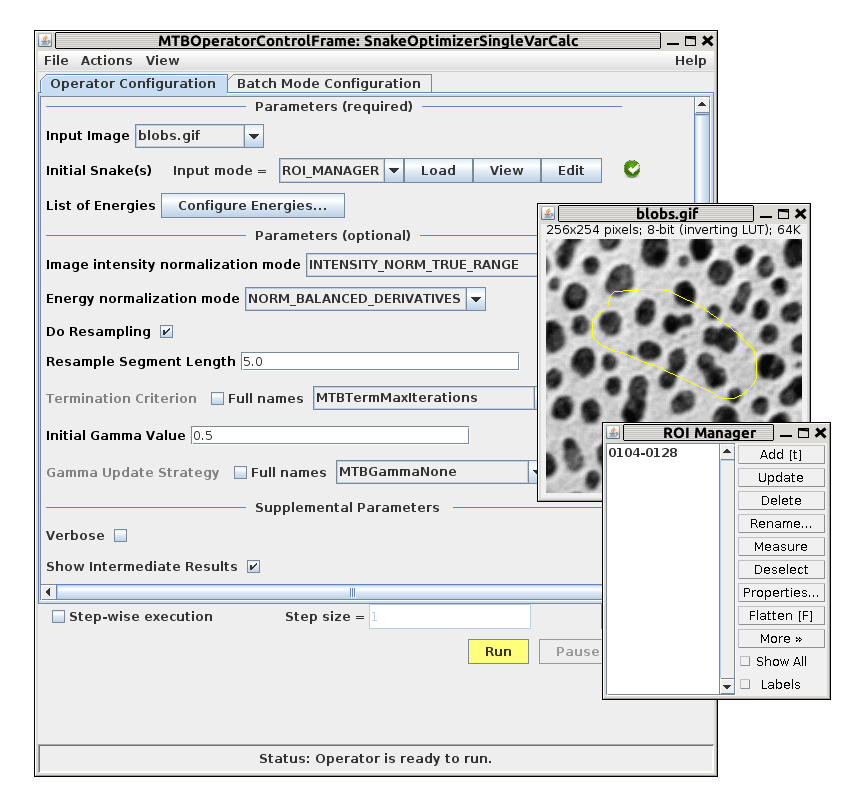
\includegraphics[width=0.6\textwidth]{../images/ScreenshotSnakeOp_trans.png}
%\caption{\label{fig:snakeop}Screenshot of the control window for the Snake Optimizer operator.}
%\end{center}
%\end{wrapfigure}
\begin{center}
\begin{figure}[t]
\begin{center}
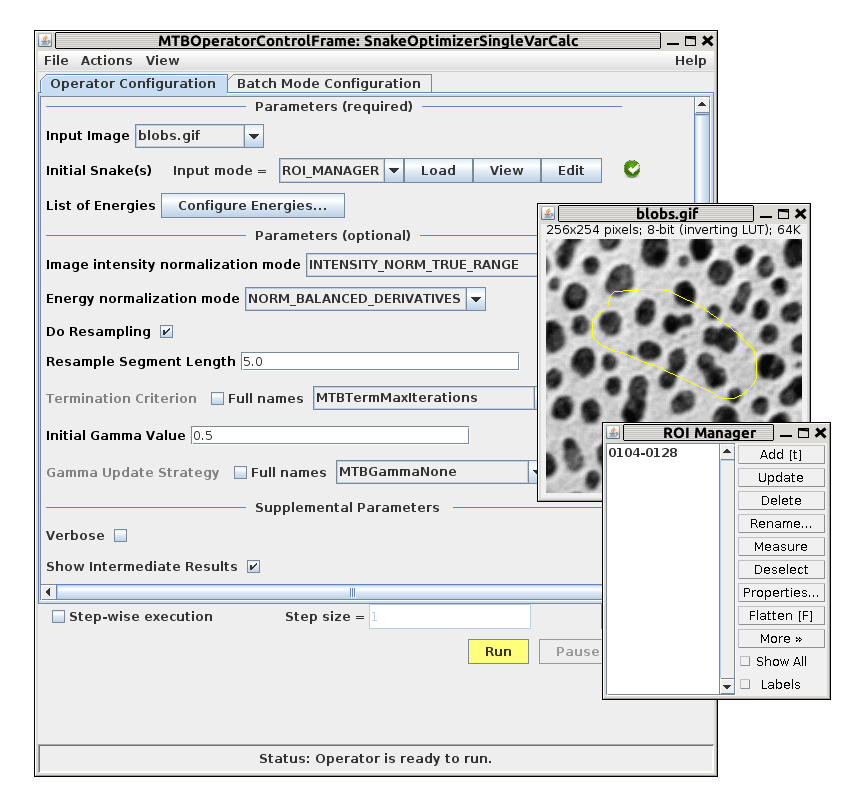
\includegraphics[width=0.85\textwidth]{../images/ScreenshotSnakeOp_trans.png}
\caption{\label{fig:snakeop}Screenshot of the control window for the 'Snake Optimizer' operator.}
\end{center}
\end{figure}
\end{center}

In Fig.~\ref{fig:snakeop} as an example the control window for the 'Snake Optimizer' operator is depicted.
It is automatically generated by the framework from the operator's source code and allows for 
operator configuration and execution. The window basically displays a panel with graphical
elements to configure all the parameters of the operator. It offers a menubar where you can 
find items for loading and saving the operator configuration, change viewing options, and also have
access to an online help for the specific operator. The help provides detailed information on the 
operator's parameters and how to configure the operator properly. The bottom section of the control
window contains control elements for executing the operator. In the simplest case there is just
a 'Run' button. More sophisticated operators, like the 'Snake Optimizer', allow for advanced user interaction.
For these operators the panel includes additional buttons, e.g., for pausing and resuming the operator. 

\label{sec:opRunImageJ}

\section{Running Operators from Commandline}
When using ImageJ or ImageJ $2.0$ it is quite natural to interact with plugins and operators, respectively, via 
graphical user interfaces. Nevertheless, quite often not only some few images need to be analyzed,
but nowadays even high-throughput processing is an important issue. While ImageJ has built-in
functionality for scripting and macros, \mitobo in addition offers a handy commandline tool by 
which all of its operators (and also ImageJ $2.0$ plugins) can directly be called from console in a
generic fashion. This way they can easily be applied to large collections of image data and also be used
from within shell scripts or comparable frameworks.  

The commandline operator runner is essentially an \alida tool, i.e.~is to be found in the package
{\tt de.unihalle.informatik.Alida.tools.OpRunner}. Its basic usage is as follows:
{\small
\begin{center}
{\tt java  de.unihalle.informatik.Alida.tools.OpRunner  <operator name>  \{
parameter=value\}}
\end{center}
}
Its first argument is the name of the operator class to be executed. You do not need to specify its complete 
package name, but the simple class name by itself is usually sufficient. Moreoever, the commandline 
operator runner also supports auto-completion if the given prefix is unique among all operators 
and plugins found on the classpath.  

Following the operator name the commandline operator runner expects a set of 'name=value' pairs 
for the parameters of the operator. While the parameter names are defined by the operator's 
member variables (execute the operator runner with option '-n' to only print its parameters), 
the exact 
syntax of the value strings depends on the data types of the parameter and their data I/O providers. 
For native data types and 
strings it is sufficient to simply provide the concrete values, for image data types a filename
is required from where to load the image. The following example illustrates this by calling 
an operator for image erosion:
{\small
\begin{center}
{\tt java de.unihalle.informatik.Alida.tools.OpRunner ImgErode inImg=test.tif
masksize=3}
\end{center}
}
However, the commandline operator runner and its built-in parser also support far more complex 
calls to operators. To illustrate this, below the call to an extended snake segmentation operator
is shown. The operator {\tt 'SnakeOptimizerCoupled'} allows to apply multiple simple snake 
optimizer operators of type 
{\tt 'SnakeOptimizerSingleVarCalc'} simultaneously to one image, given by the parameter 'inImg'. 
The operator among others takes a prototypical operator object 
of type {\tt 'SnakeOptimizerSingleVarCalc'} as input parameter ('snakeOptimizer'). This object 
by itself expects, e.g., a weighted set of energies ('energySet') which is formed by a collection 
of energy objects ('energies') and an array of corresponding weights ('weights'). The energy
objects can again be parametrized, e.g., in the example below the energy object of type 
{\tt 'MTBSnakeEnergyCD\_CVRegionFit'} defines two parameters {\tt lambda\_in} and {\tt lambda\_out}:
\begin{center}
\hspace*{-1cm}{\tt java  de.unihalle.informatik.Alida.tools.OpRunner 
SnakeOptimizerCoupled $\backslash$ }\\
{\tt  initialSnakes=RoiSet.xml inImg=cell.tif outSnakes=snakesOut.xml $\backslash$}\\
\hspace*{-1.25cm}{\tt snakeOptimizer='\$SnakeOptimizerSingleVarCalc:\{energySet= $\backslash$}\\
{\tt \{energies=[\$MTBSnakeEnergyCD\_CVRegionFit:\{lambda\_in=1.0,$\backslash$}\\
\hspace*{9cm}{\tt lambda\_out=5.0\}],$\backslash$}\\
\hspace*{-7.5cm}{\tt weights=[1.0]\}\}'}
\end{center}

For accessing the results of an operator invoked by the commandline runner it is required to 
specify targets for the operator's output parameters. In case of the image erosion operator it provides
its result through an output parameter denoted 'resultImg'. Consequently, to save the eroded image to 
file it is sufficient to extend the operator call as follows: 
\begin{center}
{\tt java  de.unihalle.informatik.Alida.tools.OpRunner ImgErode inImg=test.tif
$\backslash$\\
\hspace*{5cm} masksize=3 resultImg=result.tif}
\end{center}
Note that output parameters for which no target is provided will be ignored by the commandline 
operator runner, thus, are not available upon termination.

The examples shown above only provide you with a very brief overview of the functionality of the 
commandline operator runner. To learn more about all its options and features, please refer to 
the documentation of \alida where more details can be found.  
\label{sec:opRunCmdline}

\section{Graphical Workflow Design with Grappa}
Solving sophisticated image analysis problems usually requires to apply a combination of different
algorithms to given data to extract desired results. In ImageJ this can be
accomplished by applying a sequence of plugins sequentially or in parallel to given image data and 
record a macro of the processing steps for later reuse. \mitobo extends ImageJ's support for such 
workflows formed by multiple plugins or operators, respectively, by featuring a graphical 
editor for simplified workflow design. The editor named {\tt Grappa}, which is the acronym for 
{\em {\bf \em Grap}hical {\bf \em P}rogramming Editor for {\bf \em A}lida}, can be invoked from the plugins menu.  

In Fig.~\ref{fig:grappa} a screenshot of the Grappa main window is shown. 
The window is basically separated into
the node selection menu on the left and the workbench area on the right. In the selection menu 
all \alida and \mitobo operators (and in ImageJ $2.0$ also a subset of its plugins) are 
available as processing nodes for Grappa. The nodes in the selection menu are arranged in a 
hierarchical ordering according to their package structure. 

Workflows can be designed in the workbench area on the right. It allows to instantiate different 
workflows each being linked to an individual tab of the workbench panel. Operator nodes can be
added to a workflow either by double-clicking on the operator name in the selection menu or by 
selecting an operator and afterwards clicking once on the position in the workflow tab where the 
operator node should be positioned. Nodes can easily be dragged and repositioned as well as 
resized by mouse actions. Once different nodes have been added to a workflow, edges
can be added between ports of different nodes with the mouse to define the flow of data and control. 
All edges
are directed, always connecting an output port of one node with an input port of another. Note
that on drawing edges Grappa performs type-checking, i.e.~only ports being associated with 
compatible parameter data types can be linked to each other.
\begin{center}
\begin{figure}[t]
\begin{center}
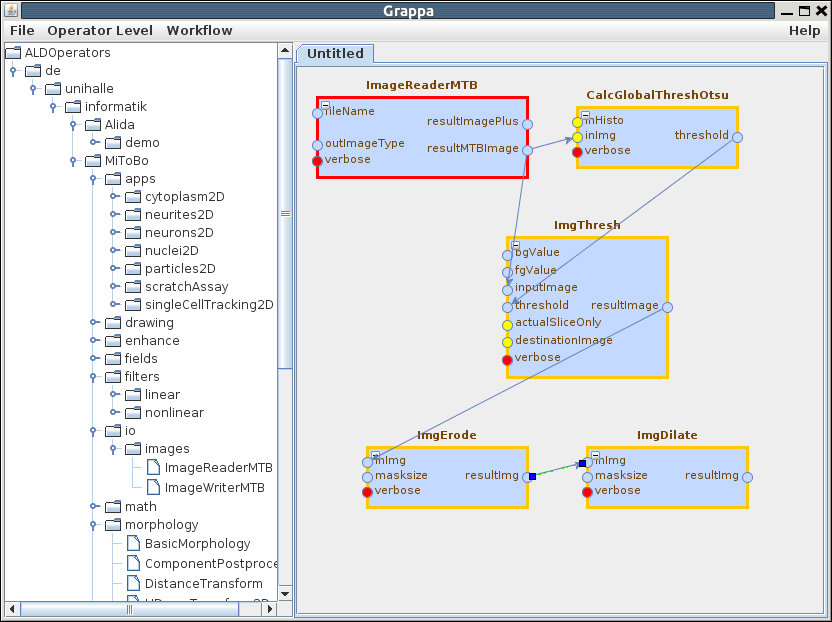
\includegraphics[width=0.85\textwidth]{../images/ScreenshotGrappa.png}
\caption{\label{fig:grappa}Screenshot of the graphical workflow editor Grappa.}
\end{center}
\end{figure}
\end{center}

\vspace*{-0.5cm}
For node configuration the mechanisms of the graphical operator runner (Sec.~\ref{sec:opRunImageJ})
are adopted. From the context menu of a node (which opens on right-clicking on the node) 
the option 'Configure\ldots' is available by which a graphical configuration window pops up.
The window is essentially identical to the control window which is displayed by the operator 
runner except that the control section is missing. All parameter values can easily be edited via
the graphical components of the window.

Nodes in a workflow can have different states indicated by the color of their border. Red framed
nodes are not ready for execution, i.e.~their configuration is not complete. If a node is readily
configured and can directly be executed its border has a yellow color, while nodes that are 
configured, however, require additional input data from preceeding operator nodes (like most of 
the nodes in Fig.~\ref{fig:grappa}) have an orange color. Prior to executing these orange nodes it
is, thus, necessary to execute the preceeding nodes first. Grappa takes care of such 
dependencies, i.e.~automatically executes nodes first from which result data is required for 
proper workflow or node execution.
After successful execution of a node its color 
changes to green indicating that result data is available. These data can graphically be examined 
via the node's context menu from which a result window can be opened. 
Note that Grappa updates the state of a node in 
real-time, i.e.~each change in its configuration or state is directly mirrored by its border color.

For executing a workflow Grappa offers different modes. Either a complete workflow can be 
executed or just a fraction of it up to a certain node. To run the complete workflow use the
corresponding item from Grappa's menubar or right-click on an empty place in the workflow tab and
select the related option from the context menu which is shown. To only partially run a workflow
select the corresponding option from the context menu of the node until which you would like to 
execute the workflow. Nodes having green color cannot be executed again until their configuration 
is changed.

Apart from the basic functionality for workflow design Grappa offers some additional convenience 
functions to simplify working with the editor. For example workflows can be saved to 
and read from disk. They can be renamed to meaningful names, and also a complete reset of a 
workflow in terms of deleting all nodes is possible. For more information on Grappa please refer
to the Alida documentation and its user and programmer guide.

\label{sec:grappa}

\section{Accessing and Exploring History Graphs}
One of the main features of \mitobo and \alida, respectively, is their capability of automatically documenting data processing
pipelines. The operator concept allows to get a detailed internal log of all data manipulations, which
can subsequently be used to convert the
process history into a directed graph data structure denoted {\em history graph} in the following.
 
The \mitobo\ operator concept defines operators as the only places where data are processed and manipulated. 
Each call to an operator is associated with a certain configuration of the operator, defined by its {\em parameters}. 
The operator receives a number of objects as input parameters, 
which for example may be images or segmentation results like regions. The behaviour of the operator is controlled by control 
parameters, for example the size of a structuring element or a threshold. 
Finally, the operator produces output data, in particular images, but also for example numerical data,
regions or contours.

In \mitobo\ an image analysis pipeline usually consists of a set of different operators that are applied to incoming data and
produce result data. The order in which the operators work on the data depends on the specific pipeline. The invocation of
operators can be of pure sequential nature or subsume parallel processing steps. In addition, a nested application
of operators is possible. Given this principle each analysis pipeline and its
data flow may be interpreted
and visualized as a directed acyclic graph (cf.~Fig.~\ref{fig:DAG} for an
example).

A \mitobo\ history graph basically consists of operator and data nodes which are connected by edges 
indicating the flow of data, as can be seen from Fig.~\ref{fig:DAG}. 
The figure shows a screenshot of \mtbc which is a graph visualization tool derived from {\em Chisio}\footnote{
Chisio website, \href{http://sourceforge.net/projects/chisio}{http://sourceforge.net/projects/chisio}}.
Chisio is a graph visualization and editing tool written in Java which we extended for the specific needs of \alida and 
\mitobo history graphs.
More detailed information about \mtbc and its installation and usage can be found on the \alida webpage and in particular 
in \alida's user guide.

Within the history graph each operator node, which is linked to the {\em call} of a specific operator,
is depicted as a rectangle with the operator's 
classname in the bottom line,
For each input and output parameter object the operator node features input and output ports which may be conceived as the entry or exit points of data into and out of the operator. These ports are depicted as filled ellipses in light green (input ports) and dark green (output ports),
respectively. Each input port has exactly one incoming edge, while an output
port may be connected to multiple target ports,
depending on where the data is passed to. In Fig.~\ref{fig:DAG} the result
image 'resultImg' produced in the {\tt MTBMedian}
operator is handed over to the {\tt ActiveContours} operator as well as
returned directly to the calling operator
{\tt CellSegmentation}. Each port of an operator has an individual name indicating the input or output object associated
with the port. This allows to distinguish between ports if one operator defines multiple input ports as is
the case for the {\tt ActiveContours} operator.
\begin{center}
\begin{figure}
\vspace*{-0.85cm}
\centerline{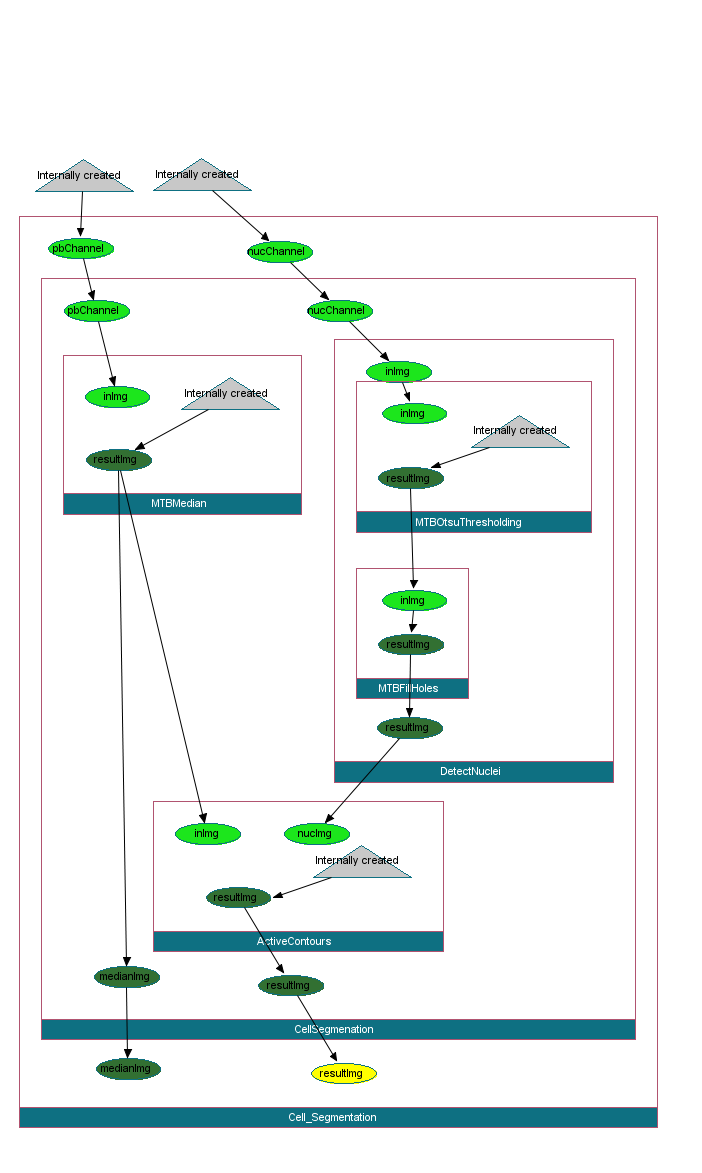
\includegraphics[clip, trim= 0 0 20 110, width=0.9\textwidth]{../images/exampleDAG.png}}
\vspace*{-0.85cm}
\caption[Example of a history graph.]{\label{fig:DAG}
A \mitobo\ history graph: the directed acyclic graph represents the application of nested operators. 
Calls to operators are depicted as rectangles, input and output ports as ellipses filled in light or dark green,
respectively. 
The grey triangles relate to newly generated data objects, and the yellow ellipse indicates the result data object
to which this history graph is linked to.}
\end{figure}
\end{center}

\vspace*{-1.25cm}
In addition to operator nodes and their ports there are also data nodes in the graph 
corresponding to the creation of new data objects, e.g., when data is read from
file, cloned or generated from scratch. These are depicted as triangles filled
in light grey.
In Fig.~\ref{fig:DAG} two data objects are created outside of the
processing pipeline as a result of reading images (at the top of the figure) and
are passed as input data objects to the {\tt Cell\_Segmentation} operator. 
Additionally, three more images are created by the operators {\tt MTBMedian}, {\tt MTBOtsuThresholding} and {\tt
ActiveContours} which in all three cases form the resulting data objects of these operators
and are passed to the outside via output ports.

Fig.~\ref{fig:DAG} shows the history graph for the output object 'resultImg' of
the operator {\tt Cell\_Segmentation}, where the corresponding port is shown as
a yellow ellipse at the bottom of the figure.
This history subsumes the calls of seven operators in total where some of these
calls are nested. The outmost operator is {\tt Cell\_Segmentation} which was
implemented as a \mitobo\ plugin, indicated by the underscore in its name
(cf.~Chap.~\ref{chap:ImplPlugins}). This plugin calls the {\tt CellSegmentation}
operator implementing the actual algorithms. For cell segmentation two input
images are required whereas one of these images is median
filtered by {\tt MTBMedian} while the second one is fed into the {\tt
DetectNuclei} operator. Inside of that operator
first {\tt MTBOtsuThresholding} is called, and the binary result image is subsequently post-processed applying {\tt
MTBFillHoles}. Its result is handed back to the calling {\tt DetectNuclei} operator and also directly propagated further back
to the {\tt CellSegmentation} operator. This operator finally calls the {\tt ActiveContours} operator which
generates one of the two result images of {\tt CellSegmentation}. The second result image is the median
filtered image which is also returned to the calling plugin as mentioned above.

The history data is stored in XML format in a file accompanying the actual data object file. 
The format basically relies on {\em GraphML}\footnote{GraphML website, 
\href{http://graphml.graphdrawing.org/}{http://graphml.graphdrawing.org/}} with some \alida and \mitobo\
specific extensions. When reading and writing images using \mitobo's {\tt 'Open\_Image\_MTB'} and {\tt 'Save\_Image\_MTB'} plugins,
or directly its {\tt 'ImageReaderMTB'} and {\tt 'ImageWriterMTB'} operators, respectively, history files are automatically considered. For example, for an image stored in the file '{\tt
example.tiff}' its history data is automatically saved to the accompanying file
'{\tt example.ald}'. The extension '{\tt
.ald}' indicates a {\em \mitobo\ processing history} file and in fact is derived from \alida, which is responsible for the 
processing histories in \mitobo. When later on reading the image using {\tt 'Open\_Image\_MTB'} or {\tt 'ImageReaderMTB'},
\mitobo's open operator checks for an accompanying file, and if one is found it is read and the corresponding history data is linked to the
image object. This allows to trace the processing history of an object in the
long run and even when the
processing pipeline was interrupted by intermediate savings of data to disk.

Note, the identity of images is {\em not} preserved in the processing history
across file boundaries. If two (or more) input images for the current top
level operator (in Fig.~\ref{fig:DAG} this would be the operator {\tt Cell\_Segmentation}), are loaded
from the same image file, both will nevertheless be displayed as different data
nodes in the history. The reason is that object identity is not -- and maybe even cannot -- be checked from the
processing history of former operations.

\paragraph{Important Note:}
At the moment, with regard to ImageJ, automatic process documentation is only supported for operators and plugins from
\mitobo\ itself, i.e.~intermediate calls to pure ImageJ functions are not documented and may corrupt the processing history. 
Contrary, in ImageJ $2.0$ also calls to ImageJ $2.0$ plugins are included in the history. But note that in both cases,
to make use of the automatic documentation to its full extent, it is indispensable to use the I/O operators of \mitobo\ to open 
input data and save the resulting output data as the ImageJ and ImageJ $2.0$ I/O functions do not know anything about histories. 

\label{sec:history}


\chapter{Configuring \mitobo}
\label{chap:config}
Several of \mitobo's operators as well as the framework itself support individual configuration by the user. For example initial
files or directories the operators should work on can be specified by the user. The probably most common way of individual
configuration is to pass specific path or flag settings to \mitobo\ operators by environment settings as outlined in this chapter.

\section{Environment Variables and Properties}
\mitobo operators support three different ways for user specific configuration:
\begin{itemize}
    \item[a)] environment variables
    \item[b)] properties of the Java virtual machine (JVM) specified with\\
     the option \texttt{'-Dproperty=value'} upon invocation of the JVM
    \item[c)] ImageJ preferences as specified in the file $\;\tilde{ }$/.imagej/IJ\_Prefs.txt\footnote{Please note that this is the
    	default configuration file of the (old) ImageJ framework, in ImageJ $2.0$ its name and place in the file system might change. 
    	Refer to the documentation of the ImageJDev project for details.} 
\end{itemize}
This order reflects the priority of the three options, i.e.~environment variables overwrite JVM
properties, and the latter ones overwrite ImageJ preferences. If for a certain operator no configuration values are
provided by any of these three ways, all default settings of the corresponding internal variables are solely 
depending on the internal settings of each individual operator.

In general there is no limitation for an operator to define configuration variables. Usually they should be properly
documented in the Javadoc of the corresponding class. Some variables of general
interest, however, are listed in the next Section \ref{sec:importantVars} as almost all users might be interested in
using them. 

The naming of the environment variables and properties is not subject to strict rules, i.e.~there are no restrictions in  
\alida/\mitobo on how to choose the names. However, it is strongly
recommended to adhere to the \alida/\mitobo naming convention as this helps to avoid
name conflicts. In \mitobo all variables start with prefix 'MITOBO'. 
Likewise in \alida all variables start with prefix 'ALIDA'. Note that some of the \alida specific
variables are also of interest in \mitobo.
The second part of the name is usually the operator class using the variable, and the third part is the actual
variable name.

\begin{center}
\fbox{\parbox{0.95\textwidth}{
\underline{Example:}\\
Imagine an operator called 'DummyOperator' which defines a variable 'Input'.\\
The environment variable that will be checked
by the operator is then

\centerline{\texttt{MITOBO\_DUMMYOPERATOR\_INPUT}}

\vspace*{0.25cm}
Obeying the naming conventions for ImageJ properties the\\
corresponding preference and also the JVM property is named\\[-0.2cm]

\centerline{\texttt{mitobo.dummyoperator.input}}
}}
\end{center}

Besides operator specific variables there may exist variables of global interest shared by different operators. In their
names the second part is simply missing, like in\\\\
\centerline{\texttt{MITOBO\_IMAGEDIR}\hspace*{1cm} or \hspace*{1cm}{\tt mitobo.imagedir},}\\\\
repectively. When defining such variables, however, special care has to be taken for
ensuring that such variables are interpreted the
same wherever they are used. And even more important, it needs to be thoroughly
verified that the variables were not
already defined elsewhere which might result in strange behavior of certain operators.

\section{List of Important Variables and Properties}
\label{sec:importantVars}
Below you find a list of variables and properties of presumably common interest.
\begin{itemize}
\item ALIDA\_OPRUNNER\_FAVORITEOPS
	\begin{itemize}
	    \item used by: {\tt ALDOpRunnerGUI}, {\tt ALDGrappaRunner}, {\tt Op\_Runner}, {\tt Grappa\_Editor}
	    \item description: configures which operators should automatically be unfolded in the operator selection menus of the 
	    	graphical operator runners and Grappa upon start-up; it should be set to a filename, and the corresponding file should 
	    	contain one operator per line, e.g.\\
	    	{\tt 
				de.unihalle.informatik.Alida.demo.ALDCalcMeanVector\\
				de.unihalle.informatik.MiToBo.tools.image.ImageDimensionReducer\\
				\ldots
				}
	\end{itemize}
\item ALIDA\_OPRUNNER\_OPERATORPATH
        \begin{itemize}
            \item used by: {\tt ALDOpRunnerGUI}, {\tt ALDGrappaRunner}, {\tt Op\_Runner}, {\tt Grappa\_Editor}
		\item	description: specifies colon separated list of packages; 
        Each package and all its sub-packages 
        is searched for operators in the classpath.
        These operators are incorporated in the tree of available operators
        in the graphical user interface.
        This feature is useful to incorporate operators which are not compiled
        but just added as within a jar-archive.
	\end{itemize}

\item ALIDA\_OPRUNNER\_LEVEL
	\begin{itemize}
	    \item used by: {\tt ALDOpRunnerGUI}, {\tt ALDGrappaRunner}, {\tt Op\_Runner}, {\tt Grappa\_Editor}
	    \item description: configures which set of operators is to be displayed initially in the selection menu; 
	    	possible options are either all available operators ('standard') or just the ones categorized as being easier 
	    	to use ('application') 
	\end{itemize}
\item ALIDA\_OPRUNNER\_WORKFLOWPATH
	\begin{itemize}
	    \item used by: all graphical and commandline operator runners, and by Grappa
	    \item description: specifies a directory where the runners are searching for additional workflows that are to be registered
	    	by the framework
	\end{itemize}
\item ALIDA\_VERSIONPROVIDER\_CLASS
	\begin{itemize}
	    \item used by: Framework
	    \item description: class used for acquiring software versions for process documentation; the class must extend the base class 
	    	{\tt ALDVersionProvider} to be found in the \alida package {\tt de.unihalle.informatik.Alida.version}  
	\end{itemize}
\item MITOBO\_IMAGEDIR
	\begin{itemize}
	    \item used by: {\tt Open\_Image\_MTB} , {\tt Save\_Image\_MTB}
	    \item description: Directory where images are expected; checked if the two variables\\
	    	MITOBO\_OPENDIR and/or MITOBO\_SAVEDIR	are not set
	\end{itemize}
\item MITOBO\_OPENDIR
	\begin{itemize}
	    \item used by: {\tt Open\_Image\_MTB}
	    \item description: directory where image browsing starts the first time 
	\end{itemize}
\item MITOBO\_SAVEDIR
	\begin{itemize}
	    \item used by: {\tt Save\_Image\_MTB}
	    \item description: directory where file selection starts the first time 
	\end{itemize}
\end{itemize}


%==================================
\part{MiToBo: The Programmer's View}
\chapter{Programming with \mitobo}
\label{chap:program}
\mitobo contains a selection of different operators for image analysis which can readily 
be applied to solve specific problems. While the first part of this guide shows how operators 
can be executed within ImageJ and via commandline, in this second part we are discussing how 
operators can be invoked on the programmatic level (Sec.~\ref{sec:callOp}). 
Moreover, we not only show how to use existing
operators, but we also introduce you to the basics of writing operators on your own 
(Sec.~\ref{sec:makeOp}). This becomes
necessary, e.g., if the existing \mitobo operators do not suit your needs, if you
would like to benefit from \mitobo's support for automatically generating graphical and 
commandline interfaces for your own algorithms, or if you would like to have your own analysis 
procedures automatically documented. Note that as \mitobo operators are basically \alida operators 
here we will focus on the substantial basics of writing \mitobo operators in the context of 
ImageJ. For more general details about implementing operators in general please refer to the 
\alida programmer's guide where much more details about \alida's concepts can be found. 

\section{Using Operators in Your Code}
\label{sec:callOp}
\alida defines a unique invocation mechanism for operators which needs to be applied when using
operators on the programmatic level. Basically the following steps are necessary to use a \mitobo
operator in your own code:
\begin{enumerate}
  \item instantiate an object of the desired operator class
  \item set the operator parameters
  \item execute the operator by calling its {\tt 'runOp(\ldots)'} method
  \item get the results
\end{enumerate}

\begin{figure*}[tbp]
\centering
\lstinputlisting[linerange={133-142},basicstyle=\small, xrightmargin=.1\textwidth,
xleftmargin=.1\textwidth]{../code/ImgOpen.java }
\caption{\label{exa:openExample}Example of a hypothetical function applying an opening to an 
image which is implemented based on \mitobo operators for morphological operations.}
\end{figure*}
In Fig.~\ref{exa:openExample} an examplary function calling \mitobo operators is shown based on 
which we will now outline the different steps listed above in detail. Suppose that the function 
that is to be realized based on \mitobo operators should perform an opening operation on an image,
i.e.~first do an erosion, then a dilation. \mitobo includes two operators for these tasks, the
erosion operator {\tt 'ImgErode'} and the dilation operator {\tt 'ImgDilate'}. Given these 
operators our opening function can be implemented as follows. First of all we instantiate an 
object of class {\tt 'ImgErode'} (line $2$ in Fig.~\ref{exa:openExample}) and specify the 
parameters using its {\tt 'setParameter(\ldots)'} method (lines $3-4$). 
The method actually takes as input the name of
the parameter to be set and the corresponding value. In line $5$ we are running the operator 
calling its {\tt 'runOp(\ldots)'} method. Note that this method is the {\em only} way of 
executing an operator. Although there are different versions of the method dedicated
to different strategies on how to document the call to the operator in the processing history
all of them basically do some logging for the processing history and then call the operator's
{\tt 'operate()'} method. Please refer to the \alida guide for further details. 

After eroding the input image we want to apply a
dilation to the result image of the erosion. To this end we instantiate an object of type
{\tt 'ImgDilate'} (line $6$). This operator class, for convenience, offers a constructor which 
already takes the parameter values as arguments. Consequently, the call of the constructor is 
sufficient in this case to readily configure the operator. In line $7$ the dilation operator is 
finally executed, and subsequently the result image is fetched from the operator and returned by
the function that was just implemented.

\section{Implementing Operators}
\label{sec:makeOp}
When the \mitobo operator runners or Grappa are required to invoke an operator, they basically 
follow the steps outlined in the previous section that have to be performed for using an operator on 
the programmatic level. First they instantiate an object of the corresponding class, then they set 
the operator's parameters to the values queried graphically or via commandline from the user,
and finally they call the {\tt 'runOp(\ldots)'} method for executing the operator. To enable this
procedure generically for all operators the implementation of an operator requires the following
things to be done:
\begin{enumerate}
  \item implementation of a public default constructor for the new operator class without any 
  	parameters as this is the only constructor of a class which can be called generically
  \item definition of the operator parameters, in \alida/\mitobo this is accomplished
  	by annotating corresponding member variables of the operator class
  \item implementation of the method {\tt 'operate()'} which should contain the functionality
  \item annotation of the operator class as a whole
\end{enumerate}
The last step is necessary to enable \alida to automatically register operators upon
start-up, e.g., to make them available to the graphical operator runner or as nodes in Grappa.

In Fig.~\ref{exa:opExample} a code snippet of a prototypical operator class is shown. The code 
is a slightly simplified version of the operator class 
{\tt 'de.unihalle.informa\-tik.MiToBo.morpholo\-gy.ImgErode'} shipped with \mitobo.

An operator in \mitobo is basically the implementation of a class extending the base class 
{\tt 'de.unihalle.informatik.MiToBo.core.operator.MTBOperator'} common for all operators (which 
by itself extends {\tt 'de.unihalle.informatik.Alida.operator.ALDOperator'}). Accordingly
from line $4$ of the code it can be seen that the new class extends \mitobo's operator base 
class. Subsequently in lines $6-16$ the parameters of the operator are declared. They are given by 
member variables annotated as {\tt 'Parameter'}. This annotation is an \alida annotation, but 
is quite similar to the corresponding annotation used in ImageJ $2.0$. The annotation requires 
for each parameter to specify a label that, e.g., is used for automatic GUI generation. In addition,
the direction of the parameter needs to be specified, i.e.~if it is an input or an output parameter,
and a short description should be given. This description is for example used to generate tooltips 
for the parameters in the operator configuration windows. 

In lines $18-24$ the default constructor of the class is implemented, while its main function is
to be found in lines $33-40$. The {\tt 'operate()'} function does the actual work. In this example 
it simply calls an internal method of the operator class (not shown for clarity), and stores the 
result of this function in the operator's output parameter 'resultImg'.

As mentioned above the operator class by itself needs to be annotated to be automatically 
registered by the \alida/\mitobo framework. This annotation can be seen in lines $2-3$. The 
annotation {\tt 'ALDAOperator'} has certain parameters, e.g.~a generic execution mode can be 
specified which allows to exclude operators from generic graphical or commandline execution. 
Also the category of the operator can be specified, i.e.~if it is easily applicable and of common 
interest, or if it is rather specialized and most probably not of common interest for most users
(cf.~Sec.~\ref{sec:opRunImageJ}).   
 \begin{figure*}[htbp]
\centering
\lstinputlisting[linerange={67-108},basicstyle=\small, xrightmargin=.1\textwidth,
xleftmargin=.1\textwidth]{../code/ImgErode.java }
\caption[Implementation example for a standard
ImageJ plugin]{\label{exa:opExample}Example implementation of an operator in \mitobo.}
\end{figure*}

On implementing a new operator you are basically free on how to organize your class. One thing 
you should keep in mind, however, is that the {\tt 'operate()'} method is the only method ever 
called on operator objects from outside (except from public getter and setter methods, if provided). 
Hence, all initialization required by the 
operator should be done within or at least be invoked from within this function, and never 
within any constructor. Finally, for improving usability of operators it is advisable,
even if not mandatory, to provide getter and setter methods for its parameters as these 
significantly simplify usage of the operator on the programmatic level.

%==================================
\section{\mitobo and ImageJ Plugins}
\label{chap:ImplPlugins}
The ImageJ plugin concept is a very powerful tool to extend the functionality of ImageJ
and, e.g., integrate third-party APIs. Accordingly, one of the main goals of the ImageJDev 
project developing ImageJ $2.0$ is to preserve the usability of available ImageJ plugins as far 
as possible. 

\mitobo seeks to extent ImageJ's functionality, 
i.e.~a natural aim is to have \mitobo operators directly available in ImageJ and ImageJ $2.0$ as
well, and to provide full integration in terms of easy interaction with other plugins. 
The straightforward solution for this goal would be to associate each single \mitobo operator with 
an explicit ImageJ $1$ or $2.0$ plugin. But, we have outlined the basic idea of generic operator 
execution implemented in \alida and \mitobo before. Consequently, as \mitobo's operator runners 
already provide functionality to execute all operators in a generic fashion, there is no need for 
explicit plugin implementations anymore. Rather it is sufficient to make the operator runners 
available as plugins in ImageJ and ImageJ $2.0$ -- which is already the case. 
Given that all operators can 
directly be used from within both ImageJ releases.

Indeed this approach of having \mitobo provide its own operator execution mechanisms also solves the
problem of compatibility to a certain degree. In particular, during the ongoing transmission period 
between both ImageJ versions it remains unclear of how to implement new plugin functionality that 
should at best be available simultaneously in ImageJ and ImageJ $2.0$. Although 
ImageJ $1$ plugins should in principal be supported by ImageJ $2$, both types of plugins are
not compatible with each other, and ImageJ $2$ plugins cannot be executed from within ImageJ $1$. 
Thus, by its operator runners being completely independent of ImageJ \mitobo offers an execution 
mechanism which is compatible with ImageJ and ImageJ $2.0$. 

Of course, this only holds if no ImageJ $1$ or ImageJ $2$ specific functionality is used by
the operators. As soon as this is done, an operator is tightly linked to one of the two ImageJ 
versions. While using ImageJ $1$ functionality might still allow to execute the operator in 
ImageJ $2$, the use of ImageJ $2$ renders the operator unsuitable for usage with ImageJ $1$.
However, this is not a \mitobo specific problem, but rather a question of software design.
Binding an implementation to an external library always renders the implementation useless without
that library. The only way to avoid such tight bindings with regard to operators and ImageJ is to
keep the functional core of operators free of ImageJ version specific dependencies as far as 
possible if the implementation targets at both releases.
 

%==================================
\chapter{\mitobo Data Types}
\label{chap:dataTypes}
\mitobo\ defines a set of its own data types. Besides new image data types
improving the ImageJ image classes, these
include for example regions and contours and some other data type primitives frequently used
with regard to image analysis applications. 
Most data types can be found in the package {\tt 'de.unihalle.informatik.MiToBo.core.datatypes'} and its
subpackages.
To allow for easy identification of the datatypes the
classnames of the data types in \mitobo\ always start with {\tt 'MTB'}, like in {\tt 'MTBRegion2D'} or {\tt
'MTBImageDouble'}.

There are several reasons why \mitobo\ implements its own data types and not
simply builds on top of the data types provided by ImageJ. First of all the handling of data objects in ImageJ is solved only in
a rudimentary fashion, at least with regard to the API. As there are only some few explicit data types apart from
images in ImageJ, data access or exchange is often cumbersome. Accordingly, \mitobo\ tries to enhance the usability and
flexibility of image processing modules by defining its own data types trying to overcome some limitations
nowadays present in ImageJ\footnote{Note that also ImageJ $2.0$ will provide a larger flexibility in data type handling, in particular 
more flexible image data types based on {\em ImgLib2}, website \href{http://fiji.sc/ImgLib2}{http://fiji.sc/ImgLib2},
will be available. Support for these extended image data types in \mitobo is planned.}.

Furthermore \mitobo defines some specific needs for data types with regard to its
feature of automatic process documentation (cf.~Sec.~\ref{sec:history}). 
Although \mitobo\ operators in principal support almost all available kinds of
objects as input and output parameters for operators, some few object
types cannot be handled natively within our concept of automatic process documentation.
Among those data types are for example Java's native data types like {\tt int} or {\tt double}, and wrapper classes like {\tt
'Integer'} and {\tt 'Double'}, i.e.~-- more generally speaking -- all
classes that implement the comparison of objects based on equality of object
values. If objects of these kinds should be used as operator input or output
parameters and, in particular, should be handed over from one operator to another, proper documentation of these data flows in the 
processing history can only be guaranteed by wrapping them in data types providing unique object identification independent of 
the current value. Accordingly, for some basic and frequently used data types \mitobo\ implements such data object wrappers.
They can be found in the package {\tt 'de.unihalle.informatik.MiToBo.core.datatypes.wrapper'}. 

Regarding automatic process documentation sometimes proper
documentation of operator configurations requires more than just logging an
input or output parameter's type and current value. There might be other object
parameters that are worth to be documented, e.g., like certain image-specific properties in case of
images. To support the documentation of such object properties \alida defines a basic data type class supporting management and
automated documentation of additional object properties. This class, {\tt ALDData}, 
serves as superclass for most \mitobo data types and can easily be adopted as basis for new data types. 

In the following sections first the properties of \alida's data type base class 
'{\tt ALDData}' will be outlined, and then we will discuss the different features and motivations 
of the most important \mitobo data types. 

\section{The Data Type Class {\tt ALDData} and its Properties}
\alida and \mitobo, respectively, allow to represent data and image processing pipelines as graph data structures, i.e.~history graphs. 
In particular, for each data object being the result of an analysis process composed of a series of data manipulations by \alida or
\mitobo operators,
the history graph allows to backtrace each single intermediate processing step subsuming all interactions with other
objects and the parameter settings of the involved operators. These data, together with the overall structure of the graph, already
draw a detailed picture of the process pipeline. However, sometimes extended information about manipulated and generated data
objects, i.e.~input and output parameters of the operators, are of interest that rise beyond the default data, like name, object
class and package. 

\alida defines the super class '{\tt de.unihalle.informatik.Alida.operator.ALDData}' to support
adding such specific information to input and output parameter objects of operators. The
class mainly adds the concept of data type {\em properties} to data types
derived from this class, allowing programmers to further characterize
objects in the processing history and also in general. Properties of
operator input and output parameter objects are automatically embedded in the history graph representation. 
Each time a data object passes an output port, i.e.~is taken out of an operator, 
the properties will be associated with the corresponding data port in the
graph. When later on viewing the graph with \mtbc (cf.~Sec.~\ref{sec:history}), the properties can then be
displayed as additional information of the corresponding ports. 

A property is basically given as a pair of key and value and is supposed to specify object characteristics. For
example in case of the \mitobo\ image data types properties subsume information like physical image and pixel sizes in all
dimensions and the units of the axes. Examplary key value pairs are shown in Table \ref{tab:propImg}.

For setting and getting object properties '{\tt ALDData}' defines two methods:
\begin{itemize}
    \item {\tt public void setProperty( String key, Object obj )}\\
    	allows to set a property named 'key' to the string representation of 'obj'
    \item {\tt public String getProperty( String key )}\\
		returns the string describing the value of the property named 'key'
\end{itemize}

Internally the properties are stored in a hashtable of the Java type {\tt 'Hashtable<String, String>'} to be found in
the package {\tt java.util}. Accordingly, keys and values are represented as strings. Nevertheless,
for convenience an arbitrary object can be handed over to the set routine as
shown above. It is automatically converted to a string via its {\tt toString()} method that consequently should return an informative description of the object at hand.
\begin{center}
\begin{table}[t]
\begin{center}
\begin{tabular}{l|l}
Property & Value \\
\hline
{\em location}  & ''/home/user/images/microscope.tif'' \\
{\em StepsizeX} & ''1''  \\
{\em StepsizeZ} & ''0.5''\\
{\em UnitX}     & ''cm'' \\
\ldots & \ldots 
\end{tabular}
\caption[Example properties of {\tt MTBImage}.]
  {\label{tab:propImg}Examplary properties and its values for an object of type {\tt MTBImage}.}
\end{center}
\end{table}
\end{center}

The programmer of a new \mitobo\ data type is in general allowed to choose arbitrary names for
the object properties without any restrictions, apart from one exception. There is one property predefined for all
\alida and \mitobo data types which is the property denoted '{\tt location}'. The location
of a data object defines the place of origin where the data object is coming from. This can be the place where it is physically stored, i.e.~the name of a
file on disk or an URL, or it can point to a virtual location if the object was generated by an operator in the course
of the processing pipeline. Note that although this property is by default
attached to all data types extending {\tt 'ALDData'}, it is, however, only set
automatically for \mitobo\ images by \mitobo's image I/O operators. For other data types setting the location
to proper values remains to the responsibility of the programmer of
the specific data type. 

To set and read the location of an object the following methods are available:
\begin{itemize}
 	\item {\tt public void setLocation( String location )}\\
 		sets the object location to the given string
    \item {\tt public String getLocation() }\\
 		returns the current location of the object 
\end{itemize} 

Note that there are no automatic checks to ensure that property names are unique. Thus, if the {\tt setProperty()} method
is called on a property which is already defined its previous value will be overwritten. This is
particularly true for the property '{\tt location}', so this key should never be
used by the programmer within another context than intended to omit confusion.


\section{Images in \mitobo: {\tt MTBImage}}
\label{sec:MTBImage}	
\mitobo defines its own image classes, namely \mtbimg~and its subclasses (which can all be found in the package
{\tt de.unihalle.informatik.MiToBo.datatypes.images}), for the following reasons:
\begin{itemize}
  \item extended pixel value precision to support all primitive numeric
  data types of Java
  \item easy access to image pixel data, but also to properties like physical pixel
  size etc.
  \item additional functionality for \mitobo's operator concept, i.e.~for documentation of
  specific image properties
\end{itemize}

In this section the internals of the \mitobo image data types are explained with more detail. The section is 
roughly divided into the following parts. At
first, some important details about the structure of \mtbimg~are given and available
image types are introduced. An overview of most common methods
for creation and manipulation of \mtbimg s follows. The section is closed
by the description of file I/O for \mtbimg~objects and how it integrates in \mitobo's
operator concept.

\subsection{The Ideas Behind \mtbimg}
\mtbimg~was not developed to fully replace ImageJ's 
\imgplus, but rather to wrap the \imgplus~objects if possible.
The most convenient way to create
a \mtbimg~from an existing \imgplus~object is to simply specify the \imgplus~as input parameter for the
method 
\centerline{\texttt{public static} \mtbimg{\tt .createMTBImage(ImagePlus img)}.}
The created \mtbimg~holds a reference to that \imgplus~object and explicitly stores the
image size as well as physical pixel size and units if available. For fast pixel
access, the \mtbimg~keeps direct references to the ImageJ data array or arrays in case
of a (hyper-)stack.

When a \mtbimg~is created from an \imgplus~the instantiated \mtbimg~must uniquely be
associated with the specified \imgplus, as no new \imgplus~is
created, but the existing one is used. This case occurs very often, e.g., when an
image window is selected from the ImageJ GUI and used as input for a \mitobo operator or plugin. 
Therefore an additional reference to the initially created \mtbimg~is added to the \textit{properties}
hashtable of the \imgplus. When an
\imgplus~with a reference to an existing \mtbimg~is passed to {\tt
createMTBImage(ImagePlus img)}, the existing \mtbimg~is simply returned.

Another aspect of \mtbimg~is to think of an \imgplus~as a 5-dimensional
image, which is the highest possible dimensionality of an image in ImageJ
(commonly denoted as 'hyperstack'). To provide easy access to higher dimensional image data
methods exist to access data in 5D hyperstacks, 3D stacks and 2D images,
which will be discussed with more detail in Section \ref{sssec:mtbimgfunc}.\\ 
\mtbimg~objects are designed in a similar way as ImageJ's \imgproc. You usually reference 
them by the abstract type \mtbimg, while one of its subclasses is actually instantiated.


\subsection{Subclasses of \mtbimg: Image Types}
One reason to develop a new image type was the limitation of ImageJ
images to 32-bit pixel value precision. The need for a 64-bit precision
floating-point image type to store results with higher accuracy was obvious.
Also the lack of a (true) 32-bit integer type in ImageJ can bear some
problems, e.g., when consecutive labels are given to image regions especially in
higher dimensional data. 

The concrete subclasses of {\tt MTBImage} indicate their types by their names. 
They share the common prefix '\mtbimg' followed by the name of the Java data type of their pixel values. 
The following list shows the image types available in \mitobo:
\begin{itemize}
  \item \mtbimg{\tt Byte} for {\tt byte}-type pixel values (unsigned as
  in ImageJ)
  \item \mtbimg{\tt Short} for {\tt short}-type pixel values (unsigned as in
  ImageJ)
  \item \mtbimg{\tt Int} for {\tt int}-type pixel values
  \item \mtbimg{\tt Float} for {\tt float}-type pixel values
  \item \mtbimg{\tt Double} for {\tt double}-type pixel values
  \item \mtbimg{\tt RGB} for three {\tt byte}-type pixel values, one
  for each color channel red, green and blue (unsigned)
\end{itemize}

All these image types share the same interface, but can be subdivided into two categories.
On the one hand there are image types that are directly linked to a corresponding ImageJ type and, thus,
simply wrap a corresponding \imgplus. On the other hander there are types that do not have a corresponding
ImageJ type. If only object references of type \mtbimg\ are used in an implementation, there is no difference 
between both classes. However, if functionality directly related to an \imgplus~object is requested or accessed 
(e.g., calls to ImageJ functions or the display of images in ImageJ's GUI), please keep in mind the differences
described in the following two paragraphs.

\paragraph{MTBImages with corresponding ImageJ types.}
If values of an \mtbimg~are changed which simply wraps the corresponding
\imgplus, the changes are directly applied to that \imgplus~as well, because 
\mtbimg~and \imgplus~share the same data arrays. Table \ref{tab:mtbimgIJ}
lists the subtypes of \mtbimg~of this category and their corresponding ImageJ image types.
\begin{table}[h]
	\begin{center}
	\begin{tabular}{|l|c|}
	\hline
	\mtbimg~subtype & \imgproc~of corresponding \imgplus \\
	\hline\hline
	\mtbimg{\tt Byte} & {\tt ByteProcessor} \\
	\hline
	\mtbimg{\tt Short} & {\tt ShortProcessor} \\
	\hline
	\mtbimg{\tt Float} & {\tt FloatProcessor} \\
	\hline
	\end{tabular}
	\end{center}
\caption{\mtbimg~types with corresponding ImageJ types.}
\label{tab:mtbimgIJ}
\end{table}

\paragraph{MTBImages without corresponding ImageJ types.}
\mtbimg s which cannot be represented by corresponding ImageJ types keep their
own data arrays and are not linked to an \imgplus~object upon creation.
Images of such data types cannot be instantiated by the {\tt createMTBImage(ImagePlus img)} method. These images are
usually constructed from scratch by specifying datatype and image size, or by
converting another \mtbimg~to that datatype.
Nevertheless, quite often an \imgplus~object needs to be associated to these images as well, usually for visualization
purposes.
\mtbimg~provides the function {\tt getImagePlus()} to obtain such an \imgplus. The
\imgplus~created is firmly associated with the \mtbimg. The new \imgplus~is of that ImageJ type which is supposed to provide the least
loss of information compared to the \mitobo source image. 
Note that \mtbimg~provides its own {\tt show()} and {\tt updateAndRepaint()} methods which already internally call the 
{\tt getImagePlus()} method. Consequently, it is not necessary to explicitly get an \imgplus~object for pure displaying purposes. \\[0.25cm]
\textbf{Important:\\
Always keep in mind, that a second image data object is kept in
memory, once {\tt getImagePlus()} or the displaying methods are called!}\\[0.25cm]
 Table \ref{tab:mtbimgNonIJ} describes the \mtbimg~types that do not have a
 corresponding ImageJ type and explains, how they are mapped to \imgplus.

\begin{table}[h]
	\begin{center}
	\begin{tabular}{|l|c|p{0.29\textwidth}|}
	\hline
	\mtbimg~subtype & \imgproc~of created \imgplus & Pixel value conversion \\ 
	\hline\hline
	\mtbimg{\tt Int} & {\tt FloatProcessor} & cast from {\tt int} to {\tt float} \\
	\hline
	\mtbimg{\tt Double} & {\tt FloatProcessor} & cast from {\tt double} to {\tt
	float} \\
	\hline
	\mtbimg{\tt RGB} & {\tt ColorProcessor} & lossless encoding of three {\tt
	byte} values to ImageJ's {\tt int} color representation \\
	\hline
	\end{tabular}
	\end{center}
\caption{\mtbimg~types without corresponding ImageJ types.}
\label{tab:mtbimgNonIJ}
\end{table}

\subsection{Construction, Data Access and Other Useful Methods of \mtbimg}
\label{sssec:mtbimgfunc} 
This subsection gives a short overview of the methods of \mtbimg~that are
widely used when working with \mitobo. A full description can be found in the
Javadoc \href{http://www.informatik.uni-halle.de/mitobo/api/index.html}{API} of \mitobo.\\[0.5cm]
At first, methods to create new \mtbimg s are presented. As there are no visible
constructors, you have to use the following {\tt static} factory functions:
\begin{itemize}
  \item {\tt public static \mtbimg~createMTBImage(\imgplus~img)}\\
  		creates a new \mtbimg~ of the correct subtype, which is uniquely linked to
  		the \imgplus
  \item {\tt public static \mtbimg~createMTBImage(int sizeX, int sizeY, int
  sizeZ, int sizeT, int sizeC, MTBImageType type)}\\
      	creates a new \mtbimg~ from scratch given the size and the data type of the
      	new image
\end{itemize}
The following methods can be used to create \mtbimg s from existing ones:
\begin{itemize}
  \item {\tt \mtbimg~duplicate()}\\
  		duplicates a \mtbimg.
  \item {\tt \mtbimg~convertType(MTBImageType type, boolean scaleDown)}\\
  		creates a \mtbimg~of the given type from the source image
\end{itemize}
There are more methods (e.g., to create a new \mtbimg~only from a part of an
existing image), please refer to the API for the other methods.

Methods for image pixel data access are declared by the \mtbimg{\tt
Manipulator} interface, which is implemented by the \mtbimg\ class. The behavior of data
access methods is similar to ImageJ's {\tt getPixel(\ldots)} and {\tt putPixel(\ldots)} methods, which
return or take a value of type {\tt 'int'} to cover 8-bit to 32-bit values. \mtbimg~provides
the same methods called {\tt getValueInt(\ldots)} and {\tt setValueInt(\ldots)}, with the only
difference that {\tt int}s are casted and not reinterpreted in case of
underlying floating point data types. Keep in mind that methods dealing with {\tt byte} types return and take values in the 
range of $[0,255]$, and methods dealing with {\tt short} types return and take values in the range of $[0,65535]$, like in ImageJ
as well. To cover floating point types additional methods
exist, which return or take {\tt double} values. These methods are called {\tt getValueDouble(\ldots)} and {\tt putValueDouble(\ldots)}. 
They define the safest way to go, if you cannot be sure which kind of images is passed to your method.

A word to (hyper-)stacks: ImageJ holds an array of 2D images, no matter if the
image is three-, four- or five-dimensional. 2D images (called 
\textit{slices} in the following) in this array (called \textit{stack}) are
referenced by $1$ to $N$, where $N$ is the total number of slices. \mtbimg~uses
indexing that every programmer is familiar with, starting from $0$ to $(N-1)$.

Below the methods to access pixel values in \mtbimg~are reviewed:
\begin{itemize}
  \item {\tt int getValueInt(int x, int y, int z, int t, int c)}\\
  		returns the pixel value at position (x,y,z,t,c) as {\tt int}
  \item {\tt void putValueInt(int x, int y, int z, int t, int c, int value)}\\
  		sets the pixel value at position (x,y,z,t,c) using an {\tt int} as input value
  \item {\tt double getValueDouble(int x, int y, int z, int t, int c)}\\
  		returns the pixel value at position (x,y,z,t,c) as {\tt double}
  \item {\tt void putValueDouble(int x, int y, int z, int t, int c, double
  value)}\\
  		sets the pixel value at position (x,y,z,t,c) using a {\tt double} as input value		
\end{itemize}

\mtbimg{\tt RGB} can be modified in the same way as color images in ImageJ, by
encoding the color values as an {\tt int} value (please refer to the ImageJ documentation for details)
and then passing that {\tt int} value to the {\tt putValueInt()} or {\tt putValueDouble()} method. 
In addition, \mtbimg{\tt RGB} further provides methods to get
and set values of the different color channels separately, or even get and work
on the \mtbimg{\tt Byte}s that represent the separate color channels.

For working with 2D images or 3D stacks there are equivalent methods that take
only 2D (i.e.~(x,y)) or 3D (i.e.~(x,y,z)) coordinates. You can also use these methods to access
certain slices (2D images) or z-stacks (3D images) of a (hyper-)stack. Therefore
you can set internal variables of \mtbimg~to specify a ``current'' slice or
z-stack with the following methods:
\begin{itemize}
  \item {\tt void setActualSliceCoords(int z, int t, int c)}\\
  		sets the coordinates of the ``current'' slice
  \item {\tt void setActualSliceIndex(int idx)}\\
  		sets the index of the ``current'' slice, i.e.~the index in the array of slices
  \item {\tt void setActualZStackCoords(int t, int c)}\\
  		sets the coordinates of the ``current'' z-stack (leaves ``current''
  		slice index unchanged)
\end{itemize}

The image data should be accessed by the above methods to develop algorithms for
generic image types. The data access methods are kept as fast as possible 
(e.g., subsume no further function calls). However, be aware that for this reason the
specified coordinates are not verified in any way. This means that running out of the
data array's bounds will cause an {\tt ArrayOutOfBoundsException} which is not caught by \mitobo.

For fast processing of higher dimensional images, you should also be aware of
how to iterate through the pixels. The usual ordering in \imgplus~hyperstacks 
is XYCZT, while \mitobo's interface
order is XYZTC. You should therefore iterate over the pixels of a \mtbimg~as
shown in the example below:\\[0.5cm]
\texttt{
\noindent\mtbimg~img = \mtbimg.createMTBImage(100, 100, 100, 100, 100,\\[-0.1cm]
						\hspace*{8.3cm}MTBImageType.MTB\_BYTE);\\[0.3cm]
for (int c = 0; c < img.getSizeC(); c++)\\[-0.1cm]
\hspace*{0.5cm}for (int t = 0; t < img.getSizeT(); t++)\\[-0.1cm] 
\hspace*{1.0cm}for (int z = 0; z < img.getSizeZ(); z++) \\[-0.1cm]
\hspace*{1.5cm}for (int y = 0; y < img.getSizeY(); y++) \\[-0.1cm]
\hspace*{2.0cm}for (int x = 0; x < img.getSizeX(); x++) \\[-0.1cm]
\hspace*{2.5cm}img.putValueInt(x,y,z,t,c,255);
}

If slicewise processing is possible, you can simply iterate over all slices,
which produces less lines of code and is the fastest way to access all
pixels:\\[0.3cm]
\texttt{
\noindent\mtbimg~img = \mtbimg.createMTBImage(100, 100, 100, 100, 100,\\[-0.1cm]
						\hspace*{8.3cm}MTBImageType.MTB\_BYTE);\\[0.3cm]
for (int i = 0; i < img.getSizeStack(); i++) \{ \\[-0.1cm]
\hspace*{0.5cm}img.setActualSliceIndex(i);\\[0.3cm]
\hspace*{0.5cm}for (int y = 0; y < img.getSizeY(); y++) \\[-0.1cm]
\hspace*{1.0cm}for (int x = 0; x < img.getSizeX(); x++) \\[-0.1cm]
\hspace*{1.5cm}img.putValueInt(x,y,255); \\[-0.1cm]
\}
}

\subsection{\mtbimg~I/O and the \mitobo~Operator Concept}
\mtbimg~extends the {\tt ALDData} base class for data types and therefore fully integrates in
\alida's and \mitobo's operator concept. 
A difference to other {\tt ALDData} types is, however, the
file input and output. \mtbimg~objects can be written to and read from disk
using the {\tt ImageWriterMTB} and {\tt ImageReaderMTB} operators, which can be
found in the package {\tt de.unihalle.informatik.MiToBo.io.images}.

The output of the save operator is comprised of two separate files: one image file in any supported
format, and a file (with ending .ald) that contains the image's processing history (see
Sec.~\ref{sec:history}). This history file -- if present -- is automatically
loaded when the image is opened using \mitobo's {\tt ImageReaderMTB} operator. The processing
history files can be examined using {\tt chipory}.

\mitobo~relies on the Bio-Formats Library
(\url{http://www.loci.wisc.edu/software/bio-formats}) and, thus, allows reading and writing
all file formats supported by Bio-Formats. Bio-Formats is a sophisticated library for image I/O
targetting at the various file formats in biomedical imaging and being compatible with the Open Microscopy Environment
(OME) standard (\url{http://www.openmicroscopy.org}).







\chapter{Useful Tools and Helper Classes}
\alida and \mitobo provide certain classes not directly related to image processing, however, useful for doing things like time
measurements or operator configuration. Such tools can usually be found in the packages {\tt de.unihalle.informatik.Alida.helpers}
and {\tt de.unihalle.informatik.MiToBo.core.helpers}, respectively.

\section{Operator Configuration}
\label{tools:plugconf}
For user specific configuration of operators \alida supports environment variables and JVM properties, while \mitobo as well supports 
ImageJ preferences (see also Chap. \ref{chap:config}). For accessing environment variables and properties/preferences \alida 
provides the class \texttt{de.unihalle.informatik.Alida.helpers.ALDEnvironmentConfig} which supports easy access to these variables
and properties. It basically defines the following methods:
\begin{itemize}
    \item {\small \texttt{public static void getConfigValue( String operator,	String propname )}}\\[0.2cm]
    	reads the value of the environment variable or property with name \mbox{'ALIDA\_operator\_propname'} or 'alida.operator.propname',
    	respectively; it follows the formerly defined 
    	priority ordering of the different configuration options, i.e.~first looks for an environment variable with the given name, 
    	then checks for JVM properties 
\end{itemize} 
If not all options should be checked, the following methods can be used alternatively:
\begin{itemize}
    \item {\small \texttt{public static String getEnvVarValue( String operator, String envVariable )}}\\[0.2cm] 
    	This method allows to directly read (only) environment variables. 
    \item {\small \texttt{public static String getJVMPropValue( String operator, String envVariable )}}\\[0.2cm] 
    	This method allows to directly read (only) JVM properties. 
\end{itemize}
\mitobo includes the class \texttt{de.unihalle.informatik.MiToBo.core.helpers.MTBEnviron\-mentConfig} extending its \alida superclass
by additional methods for accessing ImageJ properties:
\begin{itemize}
    \item {\small \texttt{public static String getImageJPropValue( String operator, String envVariable )}}\\[0.2cm] 
    	This method allows to directly read ImageJ preferences.  
    \item {\small \texttt{public static void setImageJPref( String operator, String envVar, String val )}}\\[0.2cm]
    	This method allows to set a preference in the ImageJ configuration file.
    	It is saved to the user specific ImageJ configuration file (in ImageJ usually $\;\tilde{ }$/.imagej/IJ\_Prefs.txt, but this
    	may be different in ImageJ $2.0$). Note that for actually saving the settings it is required to have the ImageJ GUI open,
    	because only on closing the GUI the preferences are actually written to the configuration file.
\end{itemize}
Note that in all cases the prefix 'mitobo.' for properties and preferences or 'MITOBO\_' for environment variables,
respectively, is internally added to the variable and property names. Likewise \mitobo overwrites the superclass methods of \alida 
as introduced above to automatically
set the \mitobo prefixes in the variable and property names. Anyway, the programmer usually does not need to pay
attention on this feature as long as he or she follows the standard naming conventions in \alida and \mitobo.



%  #]  :

\clearpage

%  #[ bibliography :

% some additional literature
%\nocite{LatexBegleiter}
%\nocite{LatexTips}

\addcontentsline{toc}{chapter}{\numberline{}Bibliography}

\bibliographystyle{alpha}
% \normalsize
% \begin{raggedright}
\bibliography{../bibfile/MiToBo_Literature}
% \end{raggedright}
% \newpage

%  #[ appendix :

\begin{appendix}

\end{appendix}

%  #]  :

\end{document}

